%\documentclass[10pt]{report}

%\usepackage[margin=2.5cm]{geometry}
%\usepackage{tikz}
%\usetikzlibrary{shapes,arrows}
%\usepackage{amsmath}
%\usepackage{array}
%\usepackage{subfigure}
%\usepackage[colorlinks=true,linkcolor=blue]{hyperref}
%%\usepackage[all]{hypcap}
%\usepackage{lscape}
%\usepackage{multirow}
%\usepackage[utf8]{inputenc}
%\usepackage[T1]{fontenc}
%\usepackage{algorithmic}
%\usepackage{algorithm}
%\usepackage{rotating}
%\setlength{\parindent}{0in}
%
%\title{Feature based classifier for Astronomical time series}
%
%\date{}
%
%\begin{document}
	%\maketitle
	
	\chapter{Baseline Features}
	\section{Aim}
		Supervised classifiers are a flexible way to incorporate many features of a data object into a classification scheme. In the context of light curve classification a variety of numerical features may be useful for discriminating between classes, from statistical properties of the flux values observed to coefficients of wavelet transforms. The aim of these experiments is to assess the transient classification performance of numerical features under a variety of single and combined distortions. The Random Forest was chosen as a classification method because of its robustness to contradictory features and overall performance. Each experiment will involve 10-fold cross validation with training features extracted from standardised light curves and tested on the remaining light curves with the distortions applied. Performance will be evaluated in terms of F-Score, Precision and Recall microaveraged across each class. The results will form a baseline of classification to which more sophisticated features and techniques will be compared.

	\section{Procedure}

	
	\subsection{Data}
	Each fold of the 10-fold cross validation will produce a training set and a test set from the raw simulation light curves, with the proportion of classes being even in each. The training set will be left as is and provided to the Random Forest to produce a set of rules. The test set will have some distortions applied according to table ~\ref{tab:experiments}. Each row of the table forms an experiment with the goal of exploring transient classification under the designated parameter values. \\

	\begin{table}[ht!]
		\label{tab:experiments}
		\centering
		\begin{tabular}{|p{0.3\textwidth}|l|p{0.45\textwidth}|} \hline
			\textbf{Experiment name} & \textbf{Distortion} & \textbf{Amounts used} \\ \hline
			Baseline & \emph{none} & \emph{none} \\
			Varying distribution & \emph{amplitude scaling} & Either \emph{centered} or \emph{-2.3 power law} \\
			Varying noise & \emph{noise} & \emph{0}, \emph{0.5}, \emph{1}, \emph{1.5} or \emph{3} signal variance added as gaussian distributed noise onto signal\\
			Varying observed data & \emph{on-line} & first \emph{10\%}, \emph{20\%}, \emph{30\%}, \emph{50\%},\emph{70\%}, \emph{90\%} datapoints available to classifier \\
			Varying missing data & \emph{missing data} & \emph{10\%}, \emph{20\%}, \emph{30\%}, \emph{50\%}, \emph{70\%}, \emph{90\%} removed randomly as 1\%, 2\%, 5\% chunks \\ \hline
		\end{tabular}
		\caption{Details of data distortion introduction}
	\end{table}
	
		\begin{table}[ht!]
		\label{tab:experiments}
		\centering
		\begin{tabular}{|p{0.3\textwidth}|l|p{0.45\textwidth}|} \hline
			\textbf{Experiment name} & \textbf{Distortion} & \textbf{Amounts used} \\ \hline
			All distortions - no missing data & \emph{on-line}, \emph{all} & first \emph{10\%}, \emph{20\%}, \emph{30\%}, \emph{50\%},\emph{70\%}, \emph{90\%} datapoints available to classifier \\ \hline
			All distortions - 1 in 10 data points missing & \emph{on-line}, \emph{all} & first \emph{10\%}, \emph{20\%}, \emph{30\%}, \emph{50\%},\emph{70\%}, \emph{90\%} datapoints available with 1 in 10 datapoints removed \\ \hline
			All distortions - 5 in 10 data points missing & \emph{on-line}, \emph{all} & first \emph{10\%}, \emph{20\%}, \emph{30\%}, \emph{50\%},\emph{70\%}, \emph{90\%} datapoints available with 5 in 10 datapoints removed \\ \hline
			All distortions - 9 in 10 data points missing & \emph{on-line}, \emph{all} & first \emph{10\%}, \emph{20\%}, \emph{30\%}, \emph{50\%},\emph{70\%}, \emph{90\%} datapoints available with 9 in 10 datapoints removed \\ \hline
		\end{tabular}
		\caption{Details of data distortion introduction}
	\end{table}
	
	\subsection{Classifier}
	The Random Forest classifier is a variant of the decision tree classifier that allows the discriminative powers of the features to be exploited more fully. Instead of a single decision tree producing a class output based on a set of rules, a series of decision trees (called a `Forest') working on a few randomly chosen features each provides a vote for the class of the subject. If a pair of features have contradictory classifications for a certain class but are good at discriminating amongst others, the Random Forest will allow them to be useful at once. \\ % TODO add a reference for decision tree, random forest, and this explanation (maybe a diagram)
	
	\subsection{Features and eliminating simulation artefacts}
	The feature sets used in the experiment are outlined in section \ref{sec:features}. Features span from basic statistical metrics (skew, kurtosis) to more sophisticated approaches used in astrophysics (periodograms and wavelet transforms). The classifier will be trained and tested on each subset as well as the whole set in order to compare classification performance and distinguish the most useful features in a practical manner. \\ \\
	With the use of simulated data care must be taken to prevent generic properties of a simulated class from leaking into the classifier. For example, if a particular class, say that of the Extreme Scattering Event (ESE) were a transient event occuring within a 200-day period, with all the other classes having time scales of 400, several features would allow to classifier to spot this arbitrary and unrealistic choice of time scales and would classify the ESE class much more accurately than it should. 
	
	\subsection{Evaluation}
	Refer to section 2. For this experiment confusion matrices will be provided for each experiment, and from these the F-Score for each class will be computed with a break down for each feature set as outlined in table~\ref{tab:features}. Additionally plots of microaveraged F-Score amongst all feature sets will be produced. F-Score is the harmonic mean of the false positive and false negative rates, both of which are vital metrics in the transient classification problem
	
	% TODO justify the Random Forest
	% TODO astronomically motivated features vs. basic statistical features, time series analysis techniques
	
	\section{Features}
	\label{sec:features}
	\subsection{Baseline feature summary}
	A summary of the baseline features and the subsets used in the experiments is given in table~\ref{tab:features}. For descriptions and discussions of each of the subsets see the following subsections. 
	The simplest features that could be useful in discriminating between light curves are metrics taken from the distribution of the flux, disregarding the time domain. Information about the variability and dynamics of a transient event is encoded in the shape of the flux histogram. In order to make the features consistent when amplitude scaling is present, feature extraction will take place after the light curve has its mean subtracted and each datapoint is divided by the standard deviation (referred to as \emph{centering}).
	
	\begin{table}
	\centering
		\label{tab:features}
	
		\begin{tabular}{|l|l|p{0.35\textwidth}|} \hline
		\textbf{Feature set} & \textbf{Short name} & \textbf{Description}\\ \hline
		\multirow{3}{*}{Basic statistical features} & \verb#stddev# & Standard deviation of flux distribution \\
		& \verb#skew# & Skew of flux distribution \\
		& \verb#kurtosis# & Kurtosis of flux distribution \\
		& \verb#beyond1std# &  Percent of flux distribution beyond one standard deviation \\ % TODO remove comments about mean, stddev
		\hline
		\multirow{5}{*}{Flux Percentiles}
		& \verb#flux_5_95# & Difference of 5th and 95th percentiles \\
		& \verb#flux_15_85# & Difference of 15th and 85th percentiles \\
		& \verb#flux_25_75# & Difference of 25th and 75th percentiles \\
		& \verb#flux_35_65# & Difference of 35th and 65th percentiles \\
		& \verb#flux_45_55# & Difference of 45th and 55th percentiles \\
		\hline
		\multirow{3}{*}{Median spreads}
		& \verb#median_deviation# & Median absolute deviation \\
		& \verb#median_buffer# & Percent of flux within 10\% of median($F$) \\
		\hline
		\multirow{2}{*}{Slope and variability}
		& \verb#amplitude_spread# & Amplitude spread \\ % TODO update code
		& \verb#max_slope# & Maximum slope over all pairs of points \\
		& \verb#slope_ratio# & Increasing / decreasing slope ratio \\
		\hline
		\multirow{1}{*}{Haar wavelet transform} & \verb#haar_coeffs(n)# for $n = 1 \ldots 15$ & Haar wavelet transform computed on centered light curve \\
		\hline
		\multirow{1}{*}{Lomb scargle periodogram} & \verb#lomb_phase(n)# for $n = 1 \ldots 4$ & Highest 4 Lomb-Scargle periodogram phase peaks \\ \hline
		\end{tabular}
		\caption{Basic feature set}
	\end{table}	
%	\subsection{Extended feature summary}
%	\begin{center}
%	\begin{tabular}{|l|l|} \hline
%	\textbf{Short name} & \textbf{Description}\\ \hline
%	\verb#grad_percentiles# & Histogram constructed from gradients sampled at particular intervals \\
%	\verb#complexity_dist# & Length of light curve divided by time scale \\
%	\verb#flux_percentiles_whole# & Flux percentiles distributed evenly from max to min, not around median \\
%	\verb#lomb_peak(n)# for $n = 1 \ldots 4$ & Size of top 4 peaks of centered light curve periodogram \\ \hline
%	\end{tabular}
%	\end{center}
	

	\subsubsection{Basic statistical features}
	\emph{Skew} and \emph{Kurtosis} are two statistical measures of the shape of a data distribution. Skew measures the degree of evenness in the distribution either side of the mean and for a set of flux values $f$ with mean $\bar{f}$ the skew is computed as:
	\begin{equation}
		\frac{\frac{1}{n}\sum\limits^{n}_{i=1}(f_{i} - \bar{f})^{3}}
		{(\frac{1}{n}\sum\limits^{n}_{i=1}(f_{i} - \bar{f})^{2})^{\frac{3}{2}}}
	\end{equation}
	
	Kurtosis measures the `peakiness' of the flux distribution - how strongly flux points are centered around the mean. For a flux sample $f$ with mean $\bar{f}$ the kurtosis is:
	\begin{equation}
		\frac{\frac{1}{n}\sum\limits^{n}_{i=1}(f_{i} - \bar{f})^{4}}
		{(\frac{1}{n}\sum\limits^{n}_{i=1}(f_{i} - \bar{f})^{2})^{2}} \\
	\end{equation}
	
	Figure~\ref{fig:samplestats} shows two sample light curves, their flux histograms and the corresponding skew and kurtosis.  It illustrates the discriminatory power of these simple features.
	Skew is highest (in magnitude) for sources with sudden pesaks and troughs emerging from background noise in one direction. As a result, the Supernovae light curve has a very positive skew. The Extreme Scattering Event has a slightly negative skew because of the relative intensity of the central dip to the peaks either side. For sources that are slowly varying or consistent, and skew will be closest to zero. \\ \\
	Kurtosis will be highest for signals that are extremely consistent or have very sudden variations. Signals that oscillate a great deal with have much lower kurtosis. Again, the supernovae, characterised by sudden sharp increases in flux, has a very high kurtosis. The ESE also has sudden variations, but not as strong as the Supernova. \\ \\
	By also computing the fraction of datapoints that lie beyond 1 standard deviation of the mean as \emph{1stddev}, the classifier can discriminate between a high kurtosis which is either the result of outliers or as the result of a very consistent signal.
		
	\begin{figure}[ht!]
		\label{fig:samplestats}
		\centering
		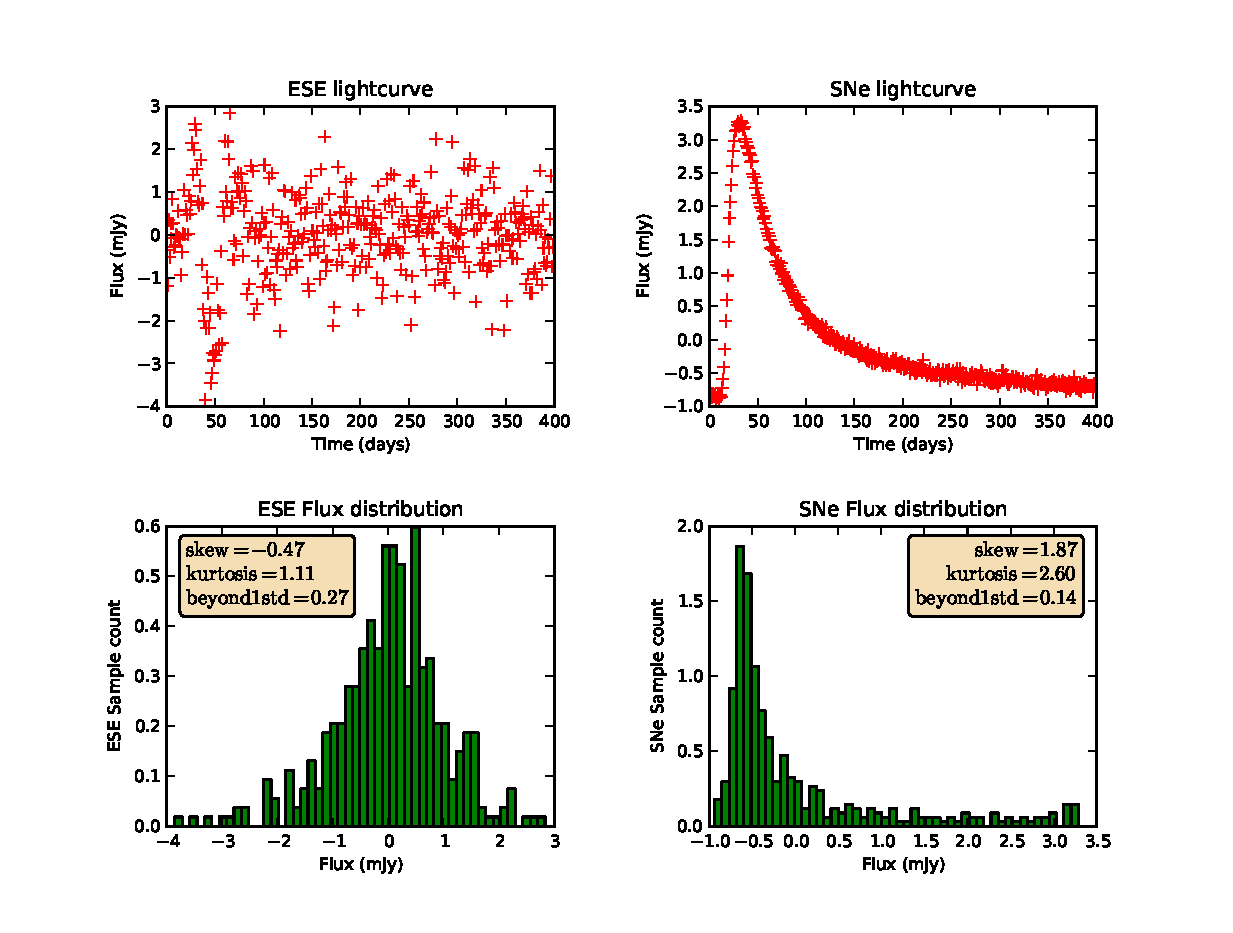
\includegraphics[width=\textwidth]{/Users/peter/honors/thesis/experiments/exp_features/figures/sample_hist.eps}
		\caption{Skewness, kurtosis, mean and standard deviation for some sample light curves}
	\end{figure}
	
	
	
	\subsubsection{Flux histogram percentiles}
	% TODO reference "Using multi-scale histograms to answer pattern existence and shape match queries over time series data"
	For most light curves the flux distribution will not be very similar to the normal distribution. As a result skew and kurtosis will be inadequate to describe the shape of the histogram. Consider figure~\ref{fig:histograms}, showing the flux distribution of an Intra-day variable (IDV) and a supernova.  \\
	
	\begin{figure}[ht!]
		\centering
		\label{fig:histograms}
		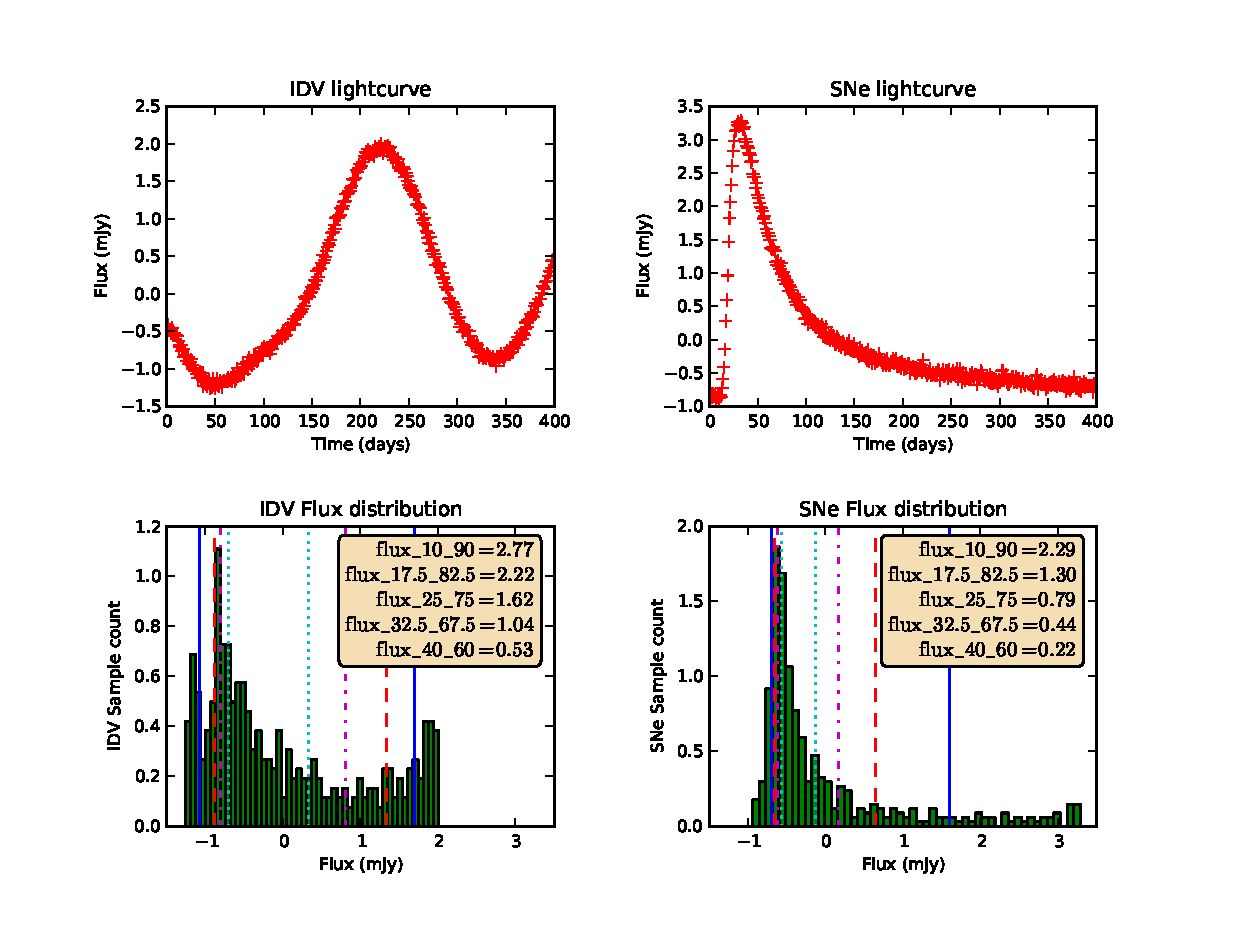
\includegraphics[width=\textwidth]{/Users/peter/honors/thesis/experiments/exp_features/figures/fluxperc_demo.eps}
		\caption{Figure of histogram feature extraction}
	\end{figure}
	
	The skew and kurtosis have little meaning for the IDV histogram, unlike for the SNe. An alternative to skew and kurtosis that will be more effective for classifying these kind of transients are extracting properties of the flux histogram at discrete intervals. A simple way to do this is to compute the differences of the sorted, standardised flux data at fixed points. These features are referred to as \emph{flux\_s\_e} with $s$ and $e$ being the percentages of the sorted flux on which the difference is computed:
	
	\begin{enumerate}
		\item Let $F$ be the vector of flux values, divided by its standard deviation and mean subtracted (centered), then \textbf{sorted}
		\item Set the difference of the 5th and 95th values from $F$ as $a$
		\item Set the difference of the 20th and 80th values from $F$ as $b$
		\item Set the difference of the 35th and 65th values from $F$ as $c$
		\item $a$, $b$ and $c$ are added as features to the classifier.
	\end{enumerate}

	
	\subsubsection{Median histogram percentiles}
	Statistical metrics that use the median of a flux distribution are typically less sensitive to noise and outlier points, one of the problems of astronomical data. Two features fall into this category: flux distribution percentiles centered on the median, and the median absolute deviation.  \\

	Median absolute deviation is defined for a centered flux distribution $f$ as:
	\begin{equation}
		\mbox{median}(\{|f_{i} - \mbox{median}(f)|\} \quad i=1\ldots\mbox{len}(f))
	\end{equation}
	The median of the set of absolute values of the flux points with the median or the original flux distribution subtracted. \\
	
	In addition to the median absolute deviation, the percentage of flux values lying within 10\% of the value of the median is used as a feature, \verb#median\_spread#.
%	The flux distribution percentiles centered on the median are computed for a centered flux distribution $f$, as:
%	\begin{enumerate}
%		\item for $m$ in [0.1, 0.25, 0.5, 0.75, 1.0, 1.5]
%		\item take percentage of points in $f$ lying within $m\cdot\mbox{median}(f)$ of median$(f)$ as feature \verb#flux_median_<m>#\
%	\end{enumerate} 
%	This is very similar to the features extracted as discrete differences of the flux distribution, except that it is more robust to noise and is better at discriminating between similar sources that are slowly varying (points clustering around the median) rather than those with sudden changes like Supernovae.
	
	\subsubsection{Slope properties}
	In an effort to include some time-domain analysis into a simple feature set, some basic properties of the slopes of the light curves was computed. These features include the most positive and the most negative slope across any pairs of time points, not considering any intermittent turning points. Another simple slope-related feature is the ratio of increasing to decreasing adjacent flux points. Although this should be useful for finding sudden changes and dramatic events, it will likely be very sensitive to noise.
	
	\begin{figure}[ht!]
		\label{fig:slopesample}
		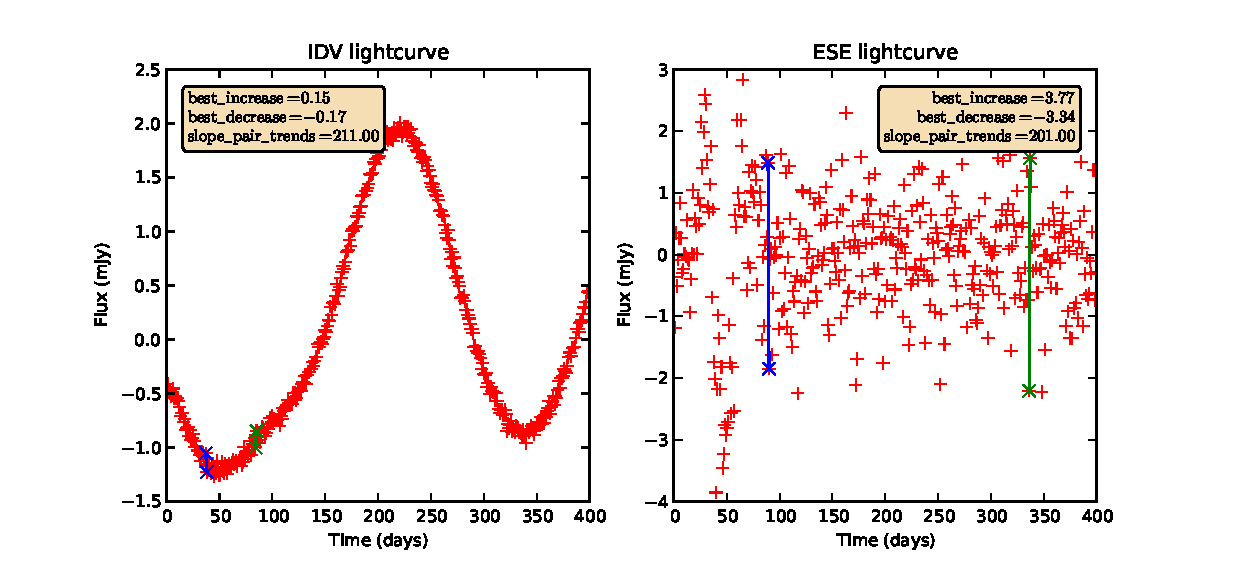
\includegraphics[height=100mm, width=\textwidth]{/Users/peter/honors/thesis/experiments/exp_features/figures/slope_demo.eps}
		\caption{Most positive (green) and negative (blue) pairwise slopes for two sample light curves}
	\end{figure}
	% TODO add justifications
	
	\subsubsection{Haar coefficients}
	The Haar wavelet transform produces a representation of the variance in a signal that is robust to noise. Square-wave shaped haar wavelets of decreasing granularity(see literature review) are fitted to data, the coefficients of each wavelet providing a means to reconstruct the original signal. Provided that the width of the signal being transformed is the same, coefficients can be compared to evaluate the similarity of a signal and its variance at different levels. \\ \\ % TODO add chapter reference
	The first 4 levels of granularity of Haar Wavelets will be used, giving 15 features in total (1 for the 1st level, 2 for the 2nd, 4 for the 3rd, and 8 for the 4th), as \verb#haar_n# for $n = 1 \ldots 15$. The transform requires that all datapoints are equally spaced in the time domain, the width of the signal is a power of 2, and there are no gaps. Both missing data and the short ends of the signal with be filled with 0s.
	
	\subsubsection{Lomb-Scargle periodogram}
	An implementation of the Lomb-Scargle periodogram based on the work in the paper \href{http://adsabs.harvard.edu/abs/1989ApJ...338..277P}{Fast algorithm for spectral analysis of unevenly sampled data} was taken from \url{http://www.astropython.org/blog/2010/9/Question-period-finding-packages-in-python}. This implementation allows us to extract as features the phase of significant peaks in the light curve and the intensity on these peaks. Computations are taken on centered (mean subtracted, divided by standard deviation) light curves and the top 5 frequences and their intensity are written as \verb#ls_phase(n)# and and \verb#ls_peak(n)# for $n = 1\ldots 5$. \\ % TODO add ref to paper
	\begin{figure}[ht!]
		\label{fig:lsspectrum}
		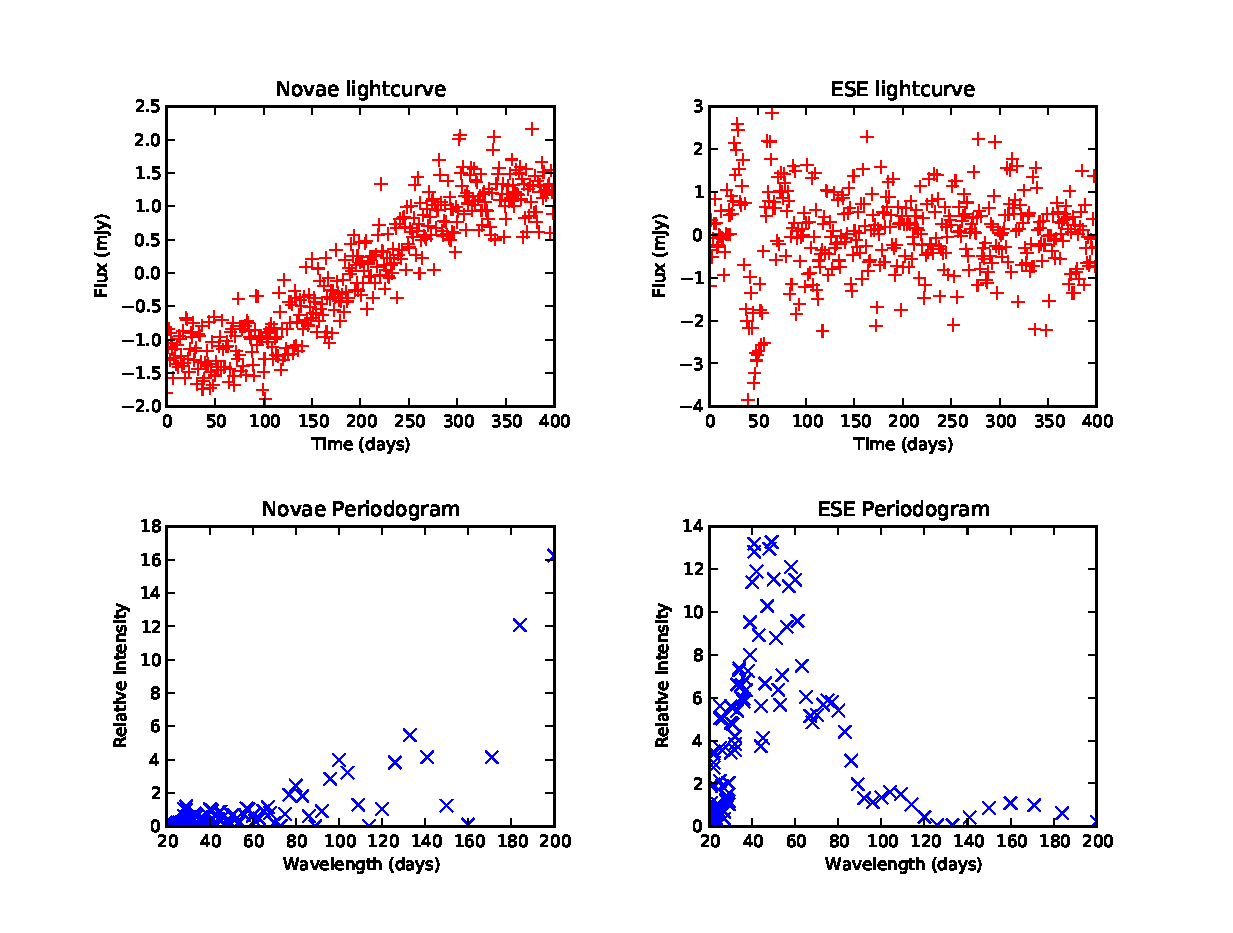
\includegraphics[width=\textwidth]{/Users/peter/honors/thesis/experiments/exp_features/figures/lomb_demo.eps}
		\caption{Spectrum produced by Lomb-Scargle periodogram for sample light curves}
	\end{figure}
	
	As they have little relation to the structure of the light curves, harmonics of wavelength less than 20 days and greater than 200 days are omitted.
	

	
	% TODO 
	%\section{Other features}
	%\begin{itemize}
	%	\item ARMA coefficients
	%	\item Distance to profile light curves under various measures
	%	\item Some kind of segmentation profile distance
	%	\item Temporal grammar distance to profiles
	%	\item Shapelet profile distance
	%\end{itemize}
		
	%\section{Results}
	%\chapter{Results} \label{chap:results}

The results go here.


%	\section{Discussion}
%	\subsection{Baseline results}
%	The baseline results for this experiment come from the classification performance trained and tested on centered lightcurves with no distortions. An additional experiment to evaluate the impact of amplitude scaling involved training on centered light curves and testing on light curves with a power law distribution, as described in chapter two. \\ \\
%	The results demonstrate that basic statistical features are very good at discriminating amongst light curves with no noise and with a consistent distribution of signal intensity. The only points of confusion with the classifer are 10\% of both the supernova and X-ray binary light curves confused with each other, and another 10\% of the supernova light curves incorrectly classified as Novae. These confusions are not surprising since in a few cases these classes look a lot like each other. Additionally, the expected inherent extreme brightness of a source like a supernova is removed as a property when the data is centered. \\ \\ % TODO is this is a valid comment?
%	The experiment evaluating classification ability under the power law distribution gives similar results. There is a slightly pronounced confusion between the supernova, X-ray binary and nova classes, most likely due to the relative slopes of the important motifs of classes between increased (or lowered) under the amplitude scaling. In addition, there is a new mutual confusion between the background source and ESE classes of about 10\%, a a misclassification of the IDV class as Novae, SNe and XRB, and finally both SNe and XRB as Flare stars. From a flux distribution only point of view, and disregarding the time domain, ESEs and BGs do have very similar light curves. It is likely that before a power law distribution the variance and distribution around the median was what distinguished these 10\% of cases. A similar explanation applies to the other issues arising in this classification. Although not a catastrophic level of confusion, it is likely these results could be improved with the use of more sophisticated features in the time domain.  \\ \\ % TODO you need evidence to support these claims
%	
%	\begin{itemize}
%		\item Breakdown per each feature, explanation of why Haar wavelets do not resolve confusion. They should be excellent features for these data conditions.
%		\item Inclusion of light curve plots for cases which were confused
%		\item Specifics of f-score, recall and precision per class
%		\item Suggestions for improvement in terms of time domain features
%	\end{itemize}
%	
%	\subsection{Varying missing data}
%	\begin{itemize}
%		\item The classifier produces an ensemble of decision trees that effectively utilises the specific class discrimination strength of each
%		\item No particular feature is good at classifying all the classes, but usually is particularly good at one. Perhaps this should be examined in more detail to give some useful insight into the features.
%		\item Spectral features performed worst, which is strange given that they should be robust to missing data
%		\item The most basic features, the statistical metrics on the flux distribution, the slope properties and the haar coefficients, performed about the same. Median based features and flux percentiles performed second worst.
%		\item  The nature of the light curve plots at the extreme end of the distortion suggests that these results - a microaveraged F-Score of 0.4 for all the features - can be improved.
%		\item Again - why do Haar coefficients perform so poorly, when they should be quite powerful for this problem?
%		\item What are some suggestions for improvements on these features, in particular extensions to the time domain.
%		\item Confusion matrices indicate that all the data appears mostly like background noise, which is expected, but more unexpectedly a lot like ESEs, and to a lesser extent flare stars and XRB. Why is this the case?
%		\item Almost no novae or supernovae are classifier correctly at even moderate amounts of missing data (5 in 10 points removed). The plots show a very clear signal even at these distortion levels, so why the decrease?
%	\end{itemize}
%	
%	\subsection{Varying observed data}
%	
%	\subsection{Varying noise to signal variance ratio}
%	
%	\subsection{Varying observed data with a power law distribution, 1.5 noise to signal variance ratio and no missing data}
%	
%	\subsection{Varying observed data with a power law distribution and 1.5 noise to signal variance ratio and 1 in 10 data points missing}
%	
%	\subsection{Varying observed data with a power law distribution, 1.5 noise to signal variance ratio and 5 in 10 data points missing}
%	
%	\subsection{Varying observed data with a power law distribution, 1.5 noise to signal variance ratio and 9 in 10 data points missing}
%	
%	
%	\section{Future work}
%	
%	\section{Conclusion}
%\end{document}
